%
% teil4.tex
%
% (c) 2023 Vincent Haufe, Hochschule Rapperswil
%
% !TEX root = ../../buch.tex
% !TEX encoding = UTF-8

\section{Lösen des Registrierungsproblems
\label{mellin:section:teil4}}
\rhead{Lösen des Registrierungsproblems}
Im ursprünglichen Problem, das uns über die letzten Abschnitte auf die 
Mellin-Transformation geführt hat, ging es ja darum, den 
Skalierungsfaktor $s$ zu finden, um den sich die beiden sonst 
identischen Funktionen $f(x)$ und $g(x)$ unterscheiden, um diese durch 
das Kompensieren mit dem Faktor $s^{-1}$ zur Deckung zu bringen.
Dies hat uns auf eine Art multiplikative Version der Kreuzkorrelation 
in Gleichung \eqref{mellin:ksigma} geführt, jedoch ist diese, wie schon 
dort erwähnt wurde, eben nicht ganz vollständig. 

Nun, da uns die Mellin-Transformation zur Verfügung steht, kennen wir 
deren Faltungs- und Korrelationsintegral.
Die Korrelation \eqref{mellin:kreuzkorrelation*} entspricht dabei bis 
auf das zusätzliche Mass $x^{-1}$ dem Integral aus Gleichung 
\eqref{mellin:ksigma}. 
Dieser Faktor lässt die Extremalstellen der Korrelation jedoch 
unverändert und findet somit den gesuchten Skalierungsfaktor $s$ unseres 
Registrierungsproblems gleichermassen.
Das nun korrekte Korrelationsintegral lässt sich über das 
Faltungstheorem der Integraltransformationen als Rücktransformation des 
Produktes der beiden Mellin-Transformierten der zu korrelierenden 
Funktionen beschreiben, völlig analog zum Vorgehen aus Abschnitt 
\ref{mellin:section:teil1}, das im ersten Beispiel auf die Lösung 
\eqref{mellin:x0ft} geführt hat, mit der einzigen Ausnahme, dass 
{\em spiegeln} im Kontext der Gruppe $(\mathbb{R^+},\cdot)$ die 
multiplikative Inversion des Arguments bedeutet:
\begin{align*}
    (f \star g)(\sigma ) 
    &= \int_\mathbb{R^+} 
    f(x) \cdot g(\sigma ^{-1} \cdot x)\,\frac{dx}{x} \\ \\
    &= \int_\mathbb{R^+} 
    f(x) \cdot g((\sigma \cdot x^{-1})^{-1})\,\frac{dx}{x} 
    = (f \ast \check{g})(\sigma)
    .
\end{align*}
Somit lautet die Lösung des Registrierungsproblems mathematisch 
ausgedrückt
\begin{equation}
    s 
    = \argmax\limits_{\sigma \in \mathbb{R^+}}
    \mathcal{M}^{-1}(\hat{f}(u) \cdot \overline{\hat{g}(u)})(\sigma)
    .
    \label{mellin:smt}
\end{equation}
Welche identisch ist zur Lösung für $x_0$ des ersten 
Registrierungsproblems, nur dass anstatt der Fourier- hier die 
Mellin-Transformation zum Einsatz kommt.

\subsection{Quantitative Bestimmung des Gewinns der Transformationsmethode
\label{mellin:subsection:gewinn}}
Das erste Registrierungsproblem mit den zueinander verschobenen 
Funktionen lässt sich sehr einfach in Python mit dem Modul {\em numpy} 
\index{numpy}
lösen. 
Dabei werden die beiden Funktionen zuerst diskretisiert indem die 
Funktionswerte für gleichmässig verteilte, diskrete $x$-Werte in ein 
Array gepackt werden.
Will man diese beiden Datenarrays nun für verschiedene 
Verschiebungswerte korrelieren, stellt {\em numpy} dafür die Funktion 
{\em convolve(f,g)} zur Verfügung. 
Durch Spiegeln der zweiten Funktion, was für das Array eine Umkehrung 
der Indizierung bedeutet, berechnet die Funktion {\em convolve()} also 
die gewünschte Kreuzkorrelation in Form eines weiteren Arrays aus, 
dessen Maximum gesucht ist und sehr einfach über Sortieralgorithmen 
gefunden werden kann. 
Die Funktion {\em convolve()} ist dabei im Hintergrund gemäss der 
diskreten Faltungsformel
\[
    (a \ast v)_n = \sum_{m = -\infty}^{\infty} a_m v_{n-m}
\]
in hoch optimiertem C-Code implementiert.
Für die in diesem Kapitel behandelte Transformationsmethode zur 
Berechnung der Korrelation sind natürlich ebenfalls Funktionen verfügbar. 
Das Modul {\em scipy.signal} bietet die Funktion {\em fftconvolve(f,g)}, 
die die übergebenen Datenarrays zuerst über den FFT-Algorithmus 
transformiert, sie anschliessend elementweise zusammenmultipliziert 
und dieses resultierende Array mit dem inversen FFT-Algorithmus wieder 
zurücktransformiert.

Mithilfe der Funktionen {\em perf\_counter()} des Moduls {\em time}, 
lassen sich beide Wege quantitativ anhand der für die Berechnung 
benötigte Rechenzeit miteinander vergleichen.
Es gilt allerdings anzumerken, dass die Resultate möglicherweise 
aufgrund der Natur von Python in ihrer Präzision und Wiederholbarkeit 
eingeschränkt und damit mit Vorbehalt zu geniessen sind.

Die Resultate sind dabei stark von den Arraygrösse und somit vom 
Grad der Auflösung der Diskretisierung abhängig.
Die Abbildung \ref{fig:mellin:zeiten} vergleicht die resultierenden 
Rechenzeiten der beiden Methoden für vier verschiedene Auflösungen.
\begin{figure}
    \centering
    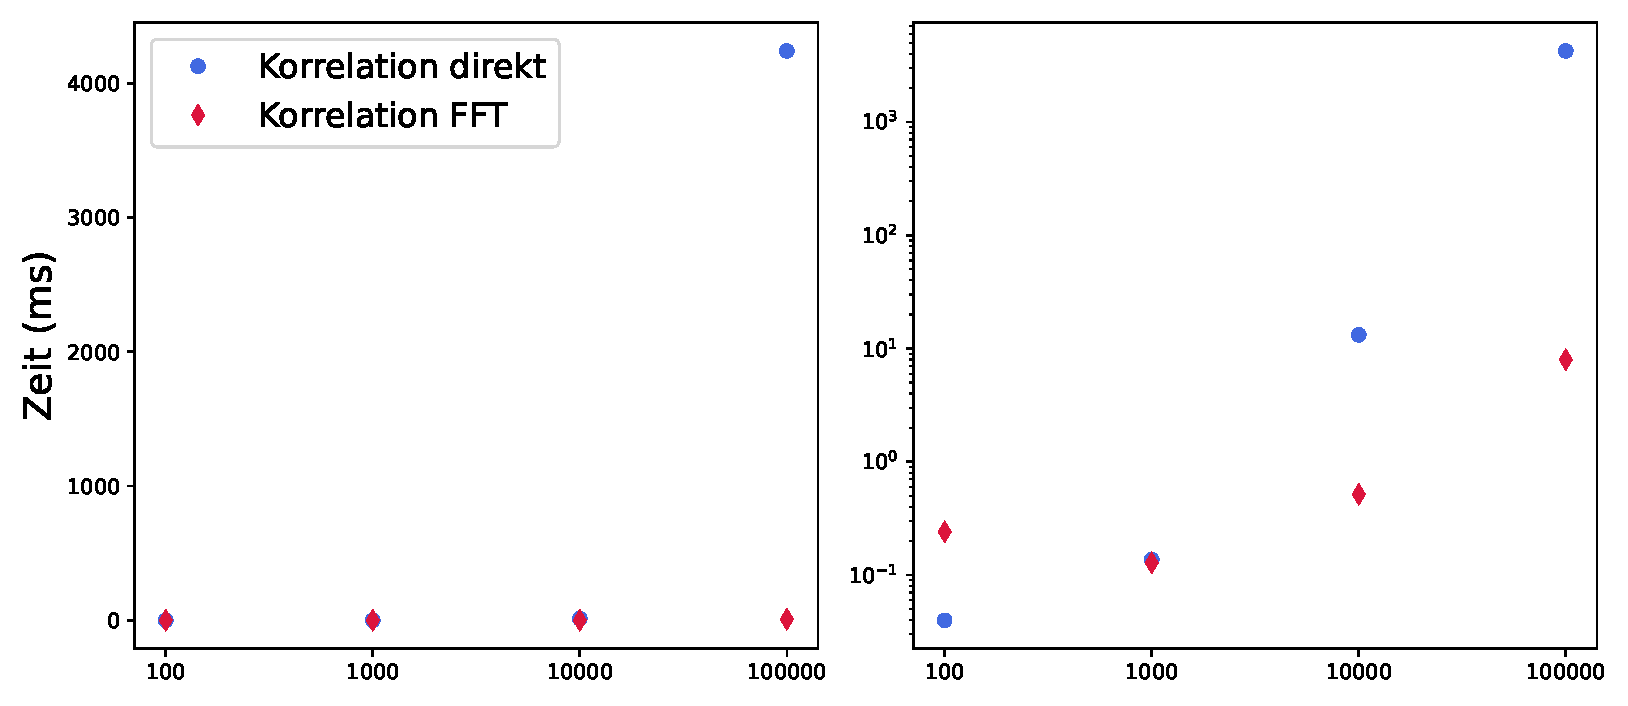
\includegraphics[width=\textwidth]{papers/mellin/images/zeiten.pdf}
    \caption{Vgl. der Rechenzeiten verschiedener Auflösungen (linear/logarithmisch)}
    \label{fig:mellin:zeiten}
\end{figure}
Wie man den Resultaten entnehmen kann, steigt die Rechenzeit der 
direkten Korrelation ab einer Auflösung von etwa 1000 Funktionswerten 
im gegebenen Intervall $x\in \left[-5,5\right]$ explosionsartig an, 
während die Rechenzeit der Korrelation über die FFT nur etwa linear 
mit der Auflösung steigt.
Hier zeigt sich also der in Abschnitt \ref{mellin:section:teil1} 
erwähnte enorme Rechenaufwand der direkten Korrelationsmethode.
Für hohe Auflösungen, die eine Anwendung meistens erfordert, ist die 
Transformationsmethode also unerlässlich.

Um auch das zweite Registrierungsproblem rechnerisch lösen zu können, 
bräuchten wir also eine diskrete Implementierung der Mellin-Transformation.
Diese könnte man wieder über die Gelfand-Theorie herleiten, als 
Transformation auf der Gruppe $(\mathbb{N}/n\mathbb{N},\cdot)$.
% https://www.researchgate.net/publication/224736063_Discrete_Mellin_transform_for_signal_analysis
Die Relationsgleichungen aus dem vorangehenden Abschnitt erlauben es uns 
aber ebenfalls, aufgrund der isomorphen Eigenschaft der 
Exponentialfunktion, erneut die FFT zu verwenden.
Das grosse Problem dabei ist aber, dass die Modifikationen, die die 
Fourier-Trans\-for\-ma\-tion in die Mellin-Transformation überführen, 
im Argument der Funktion durchgeführt werden müssen.
Bei den Datenarrays sind aber nur die Funktionswerte gegeben, und nicht 
die Funktion selbst, was es unmöglich macht die neuen Funktionswerte 
direkt aus den gegeben Funktionswerten zu bestimmen.
Indirekt kann man das Problem lösen, indem man die Funktionswerte 
geeignet interpoliert, zum Beispiel mit Splines, und die Verknüpfungen, 
die aus der Fourier-Transformation die Mellin-Transformation machen, 
auf das für die Interpolation verwendete Modell anwendet.
Dafür wäre allerdings noch einiges an Arbeit im Bereich der Numerik zu 
leisten um grundlegende Fragen zu klären, die sich bei dieser Methode 
zwangsläufig ergeben, was den Rahmen dieses Kapitels sprengen würde.
Mit diesen Ausblick auf eine ebenfalls sehr spannende Thematik im 
Bereich der Numerik soll an dieser Stelle allerdings auf eine Methode 
zur Bestimmung der diskreten, multiplikativen Korrelation mithilfe der 
harmonischen Analysis verzichten werden.


% Interpolation von f(e^t) über Splines -> auslesen an für FFT relevante Stellen 
% -> Interpolation von f(ln(t)) über Splines -> auslesen an für Korrelation relevante Stellen ODER 
%    direkt Maximum bestimmen wenn Form uninteressant, da Verknüpfung mit ln() die Extremalstellen nicht verändert


% relevante Stellen der Spline Interpolation für FFT?
% Rückgabearray der FFT? Wie hängt dies mit $\sigma$ zusammen?
% relevante Stellen der Spline Interpolation für Korrelation?


